\documentclass[a4paper]{article}
\usepackage{float}
\usepackage[spanish,es-tabla]{babel}
\usepackage[T1]{fontenc}
\usepackage[spanish]{babel}
\usepackage{graphicx} 
\usepackage[utf8]{inputenc}
\usepackage{amsmath}
\usepackage{graphicx}
\usepackage[colorinlistoftodos]{todonotes}
\usepackage[letterpaper,top=2.5cm,bottom=2.5cm,left=2.5cm,right=2.5cm,marginparwidth=2.5cm]{geometry}
\renewcommand{\baselinestretch}{1.25}


\title{Informe Física 1}
\author{Danny Córdova, Edwin Dávila}
\date{Febrero de 2023}



\begin{document}

\maketitle

\section{Introducción}
En el presente informe se abordará sobre la base de la física: la medición. El acto de medir en física se define como comparar cuantitativamente cualquier magnitud física con una unidad de un sistema de medida predeterminado. En la práctica se usó un Vernier, el cual es una herramienta de medida muy precisa y exacta, para medir las dimensiones de una esfera y de un sólido de revolución. El objetivo principal de esta práctica es revisar las bases de la teoría de medida para aprender a realizar mediciones experimentales confiables. 

\section{Metodología experimental}
Para empezar, se usó el Sistema Internacional del medidas (SI) para las mediciones, en específico, se usó el metro (m) como unidad fundamental y el milímetro (mm) como una subunidad que equivale a $10^{-3}m$. Para el cálculo de la masa, se usó igualmente el SI con el kilogramo (kg) como unidad fundamental y el gramo (g) como una subunidad que equivale a $10^{-3}kg$.  El instrumento que se usó para las medidas fue el Vernier, cuyo margen de certidumbre es de $\pm0,02 mm$. Además, para conocer la masa de los objetos se usó una balanza digital, con un margen de certidumbre de $\pm1 g$

Con ayuda del Vernier, se hicieron 30 medidas de la esfera, cada una con la esfera rotada en cierto valor para poder tener una medida más acertada. De la misma manera, se procedió con la medición del sólido de revolución para calcular su volumen. Con la balanza digital se midió la masa de los objetos. 

Las variables directas que se miden en este experimento son:
\begin{enumerate}
  \item Diámetro de la esfera (d).
  \item Diámetro de cada uno de los cilindros que componen el sólido de revolución (d).
  \item Altura de cada uno de los cilindros que componen el sólido de revolución (h).
  \item Masa de los objetos (m).
\end{enumerate}

Las variables indirectas que se calculan a partir de la información obtenida son:
\begin{enumerate}
  \item Volumen de la esfera.
  \item Volumen de cada uno de los cilindros que componen el sólido de revolución para calcular el volumen total.
  \item Densidad de los objetos.
\end{enumerate}

Las fórmulas usadas en este informe son de dos tipos: geométricas para calcular los volúmenes y estadísticas. Las fórmulas son: 

\begin{equation}
V_{esfera}=\frac{\pi}{6}d^3
\end{equation}

\begin{equation}
V_{cilindro}=\frac{\pi}{4}d^2h
\end{equation}

\begin{equation}
\Delta Z = \sqrt{{(\frac{\partial Z}{\partial A}*\Delta A)}^2+{(\frac{\partial Z}{\partial B}*\Delta B)}^2+\dots}
\end{equation}
donde $\Delta Z$ representa la propagación de incertidumbre estadística cuando se realizan varias mediciones, $\frac{\partial Z}{\partial A}$ la derivada parcial de F con respecto a A y $\Delta A$ la incertidumbre de A.

\begin{equation}
\mu= \frac{\displaystyle\sum_{i=1}^{n} x_i}{n}
\end{equation}
donde $\mu$ es la media del conjunto $x_i$ y n el número de elementos del conjunto $x_i$.

\begin{equation}
\sigma = \sqrt{\frac{1}{n-1}\displaystyle\sum_{i=1}^{n} {(x_i-\mu)}^2}
\end{equation}
donde $\sigma$ es la desviación estándar.

\begin{equation}
\varepsilon_e=\frac{\sigma}{\mu \sqrt{n}}*100\%
\end{equation}
donde $\varepsilon_e$ es el error estadístico.

\begin{equation}
\rho=\frac{m}{V}
\end{equation}
donde $\rho$ es la densidad de un cuerpo.

\begin{equation}
e=\frac{|\rho_{exp}-\rho_{teo}|}{\rho_{teo}}\times 100\%
\end{equation}
donde e es el error porcentual, $\rho_{exp}$ la densidad experimental y $\rho_{teo}$ la densidad teórica.

En la práctica se usaron 4 cifras significativas para el cálculo de los volúmenes, ya que las medidas del diámetro y la altura se podían realizar con esa precisión; y para el cálculo de las densidades se usaron solo 2 cifras significativas porque la balanza era menos precisa. 

\section{Resultados y observaciones}
Consideramos en primera instancia la incertidumbre de los instrumentos a utilizar junto a la masa de los sólidos:

\begin{table}[H]
\begin{center}
\begin{tabular}{| c | c |}
\hline
\multicolumn{2}{ |c| }{Incertidumbre instrumentos} \\ \hline
Calibrador Vernier & $\pm {0,02mm}$  \\ 
Balanza digital & $\pm {1g}$\\
\hline
\end{tabular}
\caption{Incertidumbres de los instrumentos usados en la práctica.}
\label{table:incertidumbre de instrumentos}
\end{center}
\end{table}

\begin{table}[H]
\begin{center}
\begin{tabular}{| c | c |}
\hline
\multicolumn{2}{ |c| }{Masa de los sólidos (g)} \\ \hline
Esfera & 44$\pm {1}$ \\ 
Sólido de revolución & 14 $\pm {1}$\\
\hline
\end{tabular}
\caption{Masa de los sólidos con sus incertidumbres.}
\label{tab:masa de sólidos}
\end{center}
\end{table}


Luego de usar cuidadosamente el Vernier, se obtuvieron las siguientes medias:
\begin{table}[H]
\begin{center}
\begin{tabular}{| c | c | c |}
\hline
\multicolumn{3}{ |c| }{Diámetro de la esfera (mm)} \\ \hline
22,22 $\pm {0,02}$ & 22,18 $\pm {0,02}$ & 22,20 $\pm {0,02}$\\ 
22,24 $\pm {0,02}$ & 22,18 $\pm {0,02}$ & 22,18 $\pm {0,02}$\\
22,24 $\pm {0,02}$ & 22,20 $\pm {0,02}$ & 22,20 $\pm {0,02}$\\
22,20 $\pm {0,02}$ & 22,18 $\pm {0,02}$ & 22,24 $\pm {0,02}$\\
22,26 $\pm {0,02}$ & 22,20 $\pm {0,02}$ & 22,22 $\pm {0,02}$\\ 
22,22 $\pm {0,02}$ & 22,18 $\pm {0,02}$ & 22,20 $\pm {0,02}$ \\
22,26 $\pm {0,02}$ & 22,20 $\pm {0,02}$ & 22,22 $\pm {0,02}$\\
22,22 $\pm {0,02}$ & 22,22 $\pm {0,02}$ & 22,20 $\pm {0,02}$\\
22,20 $\pm {0,02}$ & 22,18 $\pm {0,02}$ & 22,18 $\pm {0,02}$ \\ 
22,22 $\pm {0,02}$ & 22,20 $\pm {0,02}$ & 22,20 $\pm {0,02}$ \\
\hline
\end{tabular}
\caption{Diámetro de la esfera medida 30 veces.}
\label{tab:diámetro de la esfera}
\end{center}
\end{table}

Ahora con los datos del diámetro de la esfera calcularemos el valor medio:
Sumamos todos los diámetros obtenidos de la esfera $d_i$.
\[Media=\frac{\displaystyle\sum_{i=1}^{n} d_i}{n}=22.21 mm\]
Donde n=30 ya que es el número de mediciones realizadas.

Entonces el valor medio del diámetro de la esfera es de 22.21 $\pm {0,02}$ mm.

Continuamos con el volumen de la esfera, el cual se lo calcula a través de la  fórmula (1). Remplazando los datos en esta fórmula:
\[V=\frac{\pi}{6} {(22.21mm})^3=  5,736\times10^3  mm^3\] 

Ahora calculamos su debida incertidumbre a partir de la fórmula (3).
\[\Delta{V}={\frac{\partial{f}}{\partial{d}} \Delta{d}= \frac{\pi}{2} d^2\Delta{d}}\]
Reemplazamos y obtenemos que 
\[\Delta{V}= \frac{\pi}{2}(22,21mm)^2 0,02mm=\pm{1,550 \times 10^1 mm^3}\]

Entonces, el volumen de la esfera es $(5,73600\pm 0,01550)10^3  mm^3$

Se tiene el siguiente sólido de revolución:
\begin{figure}[H]
  \centering
  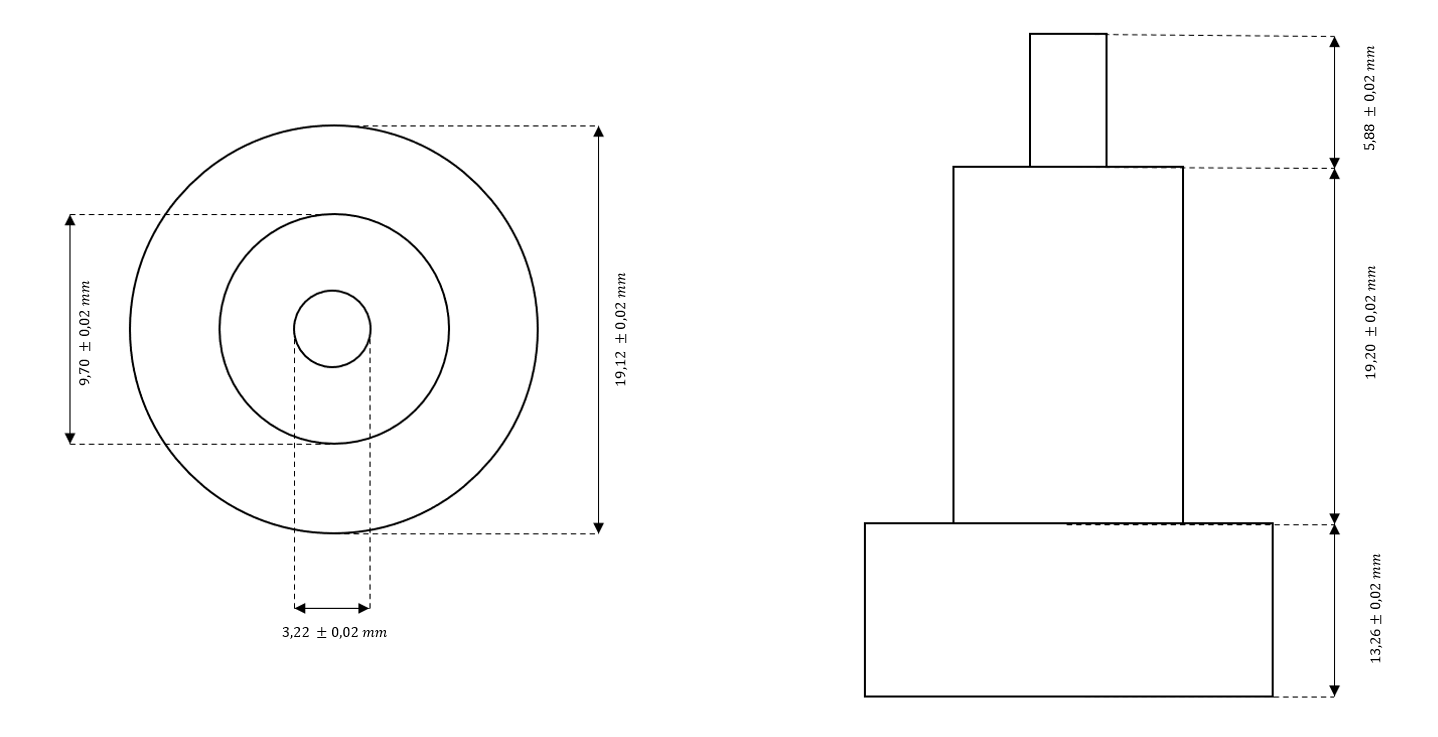
\includegraphics[width=11.5cm, height=6cm]{Solido_de_revolucion.png}
  \caption{Esbozo del sólido de revolución}
\end{figure}

Para calcular su volumen lo dividimos en 3 cilindros y usaremos la fórmula (2).
\[V_{Total}=V_1+V_2+V_3\]

\[V_1= \frac{\pi}{4}(19,12mm)^2\cdot 13,26mm=3,807
\times 10^3 mm^3\]
\[V_2= \frac{\pi}{4}(9,70mm)^2\cdot 19,20mm=1,42\times 10^3 mm^3\]
\[V_3= \frac{\pi}{4}(3,22mm)^2\cdot 5,88mm=4,79\times 10^2 mm^3\]

\[V_{Total}=(3,807\times 10^3+1,42\times 10^3+4,79\times 10^2)mm^3=5,71\times 10^3 mm^3\]

Calculamos ahora la incertidumbre del volumen del sólido de revolución usando la fórmula (3):
\[\Delta {V_{Total}}=\Delta {V_1}+\Delta {V_2}+\Delta {V_3} \]
\[\Delta{V_{Total}}= \displaystyle\sum_{i=1}^{3} \sqrt{({\frac{\pi}{2} (h_i)(d_i)(\Delta{d_i}))^2+  (\frac{\pi}{4} (d_i)^2 (\Delta{h_i}))^2}}\]

\[\Delta {V_{Total}}= 16,50 mm^3\]

Entonces el volumen del sólido de revolución es de ($5,71000 \pm {0,01650}) 10^3 mm^3 $

Ahora calculamos el error porcentual de las densidades de la esfera y del sólido. Considerando que el sólido es de aluminio y la esfera es de acero, se calculan respectivamente sus densidades, a través de la fórmula (7) y se encuentran los errores porcentuales a través de la fórmula (8):
Densidad del sólido:
\[p_{exp}=\frac{14g}{5,71\times 10^3 mm^3 }= 2,5 \times 10^{-3} \frac{g}{mm^3}=2,5\frac{g}{cm^3}\]
Usando la fórmula (3), calculamos la incertidumbre:
\[\Delta \rho=\sqrt{({\frac{1}{V}(\Delta{m}))^2+  (-\frac{m}{V^2} (\Delta{V}))^2}}\]
\[\Delta \rho=0.18 \frac{g}{cm^3}\]
Entonces la densidad del sólido es: $(2,50\pm0.18) \frac{g}{cm^3}$.

Densidad de la esfera:
\[p_{exp}=\frac{44g}{5,736 \times 10^3 mm^3}= 7,7 \times 10^{-3} \frac{g}{mm^3}=7,7\frac{g}{cm^3}\] 
Usando la fórmula (3), calculamos la incertidumbre:
\[\Delta \rho=\sqrt{({\frac{1}{V}(\Delta{m}))^2+  (-\frac{m}{V^2} (\Delta{V}))^2}}\]
\[\Delta \rho=0,23 \frac{g}{cm^3}\]
Entonces la densidad de la esfera es: $(7,70\pm0.23) \frac{g}{cm^3}$.

Considerando que la densidad del aluminio es de 2,70 $\frac{g}{cm^3}$ y la del acero es de 7,80 $\frac{g}{cm^3}$.

Entonces tenemos el error porcentual del volumen del sólido a partir de la fórmula (8):

\[e=\frac{|2,50 - 2,70|}{2,70}\cdot 100 \%=7.41\%\]

De igual forma, repetimos el proceso con los datos de la esfera.

\[e=\frac{|7,70 - 7,80|}{7,8}\cdot 100 \%=1,28\%\]

\section{Conclusiones}
Mediante la presente práctica se pudo corroborar la importancia que tienen las mediciones en la física. Estas permiten que la física experimental (y por lo tanto la física en general) avance, ya que el proceso de medición comprueba que una teoría o modelo físico sea consistente con lo observado en la realidad. Un hecho importante que cabe recalcar es que mientras mayor sea el número de medidas sobre una magnitud, más precisa será la media de la medida y por lo tanto su incertidumbre será menor. Esto se puede comprobar con los errores porcentuales de densidad calculados en la práctica: la esfera fue el objeto que más veces se midió y el que obtuvo un error porcentual menor a comparación del sólido de revolución ($1,28\%$ en comparación con  $7,41\%$). 


\section{Referencias}
\begin{enumerate}
    \item Grefa, J., Herrera, N., \& Procel, L. (2019). \textit{Mediciones y propagación de errores}.
\end{enumerate}


\end{document}
